{
{\sffamily Dette afsnit har til formål at beskrive hvordan vi trækker
regioner ud af billedet. Kort sagt forsøger vi at segmentere billedet
ved primært ved at bruge en metode kaldet floodfill. Vi præparerer dog
først billedet ved at finde kanter og sløre billedet. Vi vil også komme
ind på hvilke andre metoder vi har forsøgt os med. Først vil vi dog se
på hvilke tanker vi har gjort os om valg af programmeringssprog og
implementationen generelt.
%navnligt den funktion i OpenCV der er buggy, GoodFeaturesToTrack og
%Perona and Malik fra Octave. Det følgende afsnit om Floodfill bør være
%en del af dette afsnit, ligesom vi skal have lignende beskrivelser af
%sløring og kant detektion.
}

\subsection{Programmeringssprog og biblioteker}
Ved valg af programmeringssprog har vi først og fremmest lagt vægt på at
kunne udarbejde en prototype hurtigt og have et sprog som er let at gå
til. Det valgte sprog skal også gøre det nemt at udvide den endelige
implementation. Vi har også gerne ville undgå at skulle konstruere
komplicerede datastrukturer for relativt simple metoder, både af hensyn
til tidspres, men også til implementationens kompleksitet. Af
ovenstående grunde har vi besluttet at udarbejde vores løsning i
programmeringssproget Python, da netop dette sprog er yderst velegnet
til at skrive forholdsvis avancerede prototyper i. Python er
ydermere meget fleksibelt med hensyn til datastrukturer og byder
umiddelbart på en lang række pakker relevant for problemstillingen.

(Skal man skrive noget om Pythons udbredelse, anerkendelse og brug?)

\subsubsection*{OpenCV}
Til at udføre billedmanipulation benytter vi os af et bibliotek skrevet
i C og C++ der hedder \emph{OpenCV}. Biblioteket er udviklet af Intel og
tilbyder, udover et solidt udvalg af algoritmer, bindinger til Python.
Endelig er det meget veldokumenteret og giver referencer til
publikationer om bibliotekets algoritmer. Biblioteket er udviklet med
specielt henblik på real-tids behandling af billeder, f.eks. med et
videokamera som kilde, men egner sig også til brug på enkelte billeder.
\emph{OpenCV} tilbyder mange brugbare datastrukturer med hensyn til
arbejdet med billeder i Python.

Der tilbydes også andre biblioteker til billedbehandling i Python. Her
kan nævnes \emph{PIL} (Python Image Library) og \emph{PythonMagick}
(ImageMagick bindings), men de er ikke nær så grundige som
\emph{OpenCv}. Der findes dog metoder i \emph{OpenCV} til at samarbejde
med \emph{PIL}, men vi har ikke set det nødvendigt at udnytte dette.

%\subsubsection*{SQLite}
% Der snakkes om dette i Opbevaring af billeder, mon ikke det er nok?

\subsubsection{Alternative muligheder}
Der er to helt oplagte mugligheder med hensyn til programmeringssprog
når man taler om billedbehandling, nemlig Matlab og dets Open
Source-alternativ Octave. De blev dog valgt fra, da vores samlede
erfaring med udvikling i disse sprog ikke var stor nok. Endvidere, selv
om de især egner sig til de beregninger vi skal lave, så finder vi at
disse sprog besværlige at lave større programmer med. Matlab og Octave
er dog blevet brugt til at sammenligne resultater og teste alternative
metoder med. Dette vil vi vende tilbage til.

Da \emph{OpenCV} er skrevet i C/C++ ville det også være oplagt at bruge et af
disse sprog. Vores erfaring er dog, at man let kommer til at bruge mere
tid på at konstruere de fornødne datastrukturer og hjælpemetoder hvilket
let flytter fokus fra opgavens kerne. En senere implementation, med
fokus på køretid, kunne med fordel implementeres i C/C++, da man vil
have fuld kontrol over hvilke strukturer der bliver brugt i programmet.

\subsection{Kantdetektion}
Indsæt beskrivelse af kantdetektion.

\subsection{Sløring}
Indsæt beskrivelse af sløring (blur).

\subsection{Floodfill}
% Denne fil er inkluderet i udtraekning_af_regioner.tex
{

Floodfill finder de områder i et billede, hvis farve ligger inden for en
vis afvigelse af den originale farve. Der vælges en pixel i billedet,
som har en farve angivet ved en RGB-værdi. Ud fra denne pixel findes de
fire tilstødende pixels i lodret og vandret bane, som vist i figur
\ref{floodfill1}.

\begin{figure}[!h]
    \begin{center}
        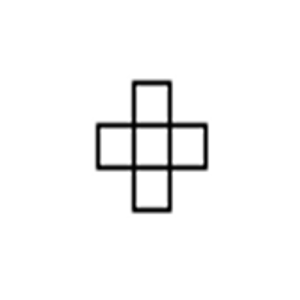
\includegraphics[scale=0.42,angle=0]{afsnit/vores_implementation/billeder/flood_fill/floodfill1}
    \end{center}
    \caption[]{Måden hvorpå floodfill arbejder med pixels i billedet.}
    \label{floodfill1}
\end{figure}

\subsubsection{Metode}
De følgende 3 skridt beskriver, hvordan floodfillmetoden virker i et
billede.

\begin{enumerate}
    \item Algoritmen starter med at markere den midterste pixel (vores
        startpixel) med et rødt flag, som angiver, at denne pixel bliver
        farvet. Nabopixels får et blåt flag, som angiver, at de skal
        kontrolleres for, om deres farve er inden for afvigelsen. Blå
        flag sættes kun, hvis en pixel ikke har noget flag i forvejen.
        Se figur \ref{floodfill2}.
    \item Hver pixel med et blåt flag kontrolleres for, om deres farve
        ligger indenfor afvigelsen. Hvis farven er inden for afvigelsen,
        bliver denne pixel sat i en liste og markeret med et grønt flag
        og et tal. Se figur \ref{floodfill3}.
    \item En pixel med grønt flag tages ud af listen og bliver sat til
        den nye startpixel. Skridt $1$ og $2$ bliver gentaget, til der
        ikke er flere grønne flag. Se figur \ref{floodfill4}.
\end{enumerate}

\begin{figure}[!h]
    \begin{center}
        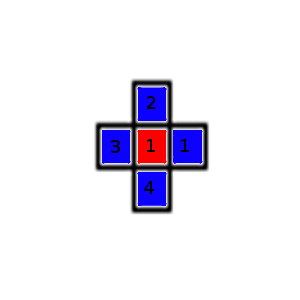
\includegraphics[scale=0.42,angle=0]{afsnit/vores_implementation/billeder/flood_fill/floodfill2}
    \end{center}
    \caption[]{Pixels efter første skridt i algoritmen. Den røde pixel
    er vores startpixel. Pixels, markeret med blåt, skal kontrolleres for
    deres farve. Numrene angiver rækkefølgen hvori de bliver gennemgået.}
    \label{floodfill2}
\end{figure}

\begin{figure}[!h]
    \begin{center}
        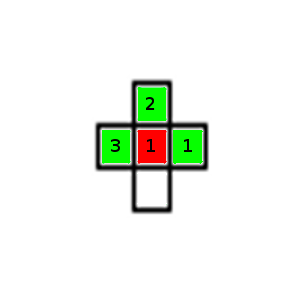
\includegraphics[scale=0.42,angle=0]{afsnit/vores_implementation/billeder/flood_fill/floodfill3}
    \end{center}
    \caption[]{Pixels efter andet skridt i algoritmen. De pixels, som har
    en farve, der ligger inden for afvigelsen, bliver markeret med et grønt
    flag og tildelt et tal, som angiver rækkefølgen. I denne illustration
    er den nederste pixel ikke blevet farvet grøn. Den var før blå, men
    da den ikke ligger inden for afvigelsen, mister den sit flag.}
    \label{floodfill3}
\end{figure}

\begin{figure}[!h]
    \begin{center}
        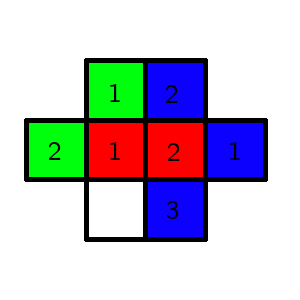
\includegraphics[scale=0.42,angle=0]{afsnit/vores_implementation/billeder/flood_fill/floodfill4}
    \end{center}
    \caption[]{Pixels efter skridt tre og et nyt skridt 1. Vi har valgt
    den grønne pixel, med det laveste tal, fra figur \ref{floodfill3} som
    ny startpixel. Nye pixels markeret med blåt mangler at blive
    kontrolleret.}
    \label{floodfill4}
\end{figure}

På denne måde itererer metoden sig igennem alle de pixels, som ligger
inden for en vis afvigelse fra startfarven. Metoden kan bruges på to
måder; enten kan man regne varianten fra den første startpixel ud, og
således kun have én startfarve, eller man kan ændre den efter den nye
startpixel --- som bliver fundet i tredje skridt --- og således have en
startfarve, der ændres efterhånden. Det skal bemærkes, at den pixel, som
i figur \ref{floodfill3} mister sit blå flag, godt kan blive taget i
betragtning igen senere, når vi vælger en ny startpixel. En pixel kan
dog højst blive taget i betragtning i alt fire gange, fordi den har fire
tilstødende pixels.

\subsubsection{Eksempler}
Vi vil nu eksemplificere, hvordan denne metode virker i praksis ved
manipulation af billedet vist i figur \ref{bathers}.  Dette billede er
valgt, da det har været brugt i flere argumenter for, at man i
malerkunsten finder særligt mange interessante regioner i det gyldne
snit\cite{GoldenNumber,RatioArt}. Endvidere er maleriet
interessant at teste på, da det er udført i det, der kaldes
pointilistisk stil, hvilket vil sige, at maleriet faktisk består af en
masse små prikker. I de fem billeder vist i figur
\ref{dot_ff_fixed_7_7}, \ref{dot_ff_var_7_7}, \ref{dot_ff_fixed_10_10},
\ref{dot_ff_var_10_10} og \ref{dot_ff_var_9_9} bruges floodfill på den
pixel, der er at finde i midten af den røde prik. Den tilladte afvigelse
gives som parret $(lo, up)$ med en værdi for, hvor meget RGB-værdien må
henholdsvis falde og stige. Det anbefales at studere figurene og den
tilhørende tekst.

% Det her billede opfører sig underligt mht. scale :/
\begin{figure}[!h]
    \begin{center}
        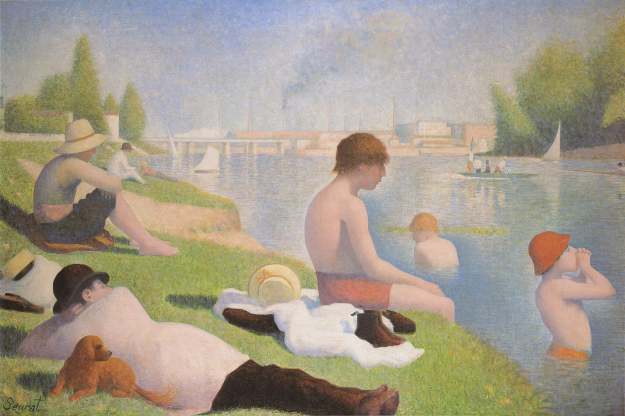
\includegraphics[scale=8]{afsnit/vores_implementation/billeder/flood_fill/seurat_bathers}
    \end{center}
    \caption[George Seurat: \emph{Bathers at Asnieres} -- 1884]{George
    Seurat: \emph{Bathers at Asnieres} - 1884\\Originalt billede.}
    \label{bathers}
\end{figure}

\begin{figure}[!h]
    \begin{center}
        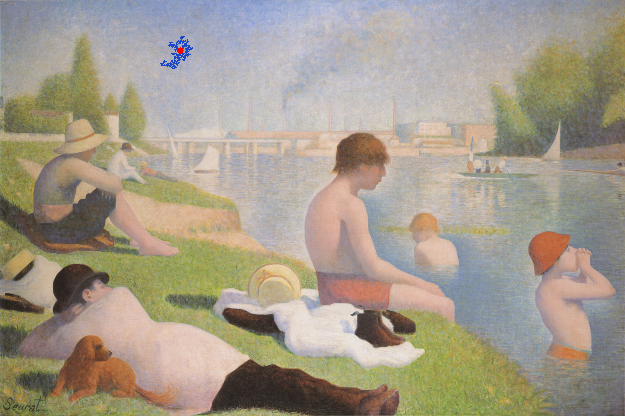
\includegraphics[scale=0.49]{afsnit/vores_implementation/billeder/flood_fill/dot_ff_fixed_7_7}
    \end{center}
    \caption[]{Floodfill-metoden i et billede, hvor der kun sammenlignes
    med farven på den originale pixel med afvigelsen $(7,7)$.}
    \label{dot_ff_fixed_7_7}
\end{figure}

\begin{figure}[!h]
    \begin{center}
        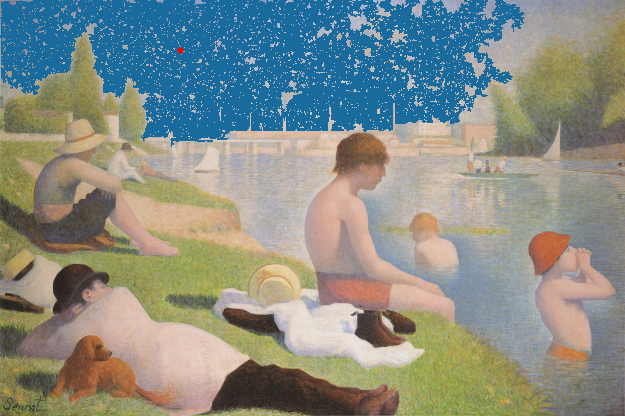
\includegraphics[scale=0.49]{afsnit/vores_implementation/billeder/flood_fill/dot_ff_var_7_7}
    \end{center}
    \caption[]{Floodfill-metoden i et billede, hvor der sammenlignes med
    farven på den nye startpixel. Afvigelsen er sat til $(7,7)$ ligesom
    i figur \ref{dot_ff_fixed_7_7}. Det ses, at vi nu dækker et meget
    større areal.}
    \label{dot_ff_var_7_7}
\end{figure}

\begin{figure}[!h]
    \begin{center}
        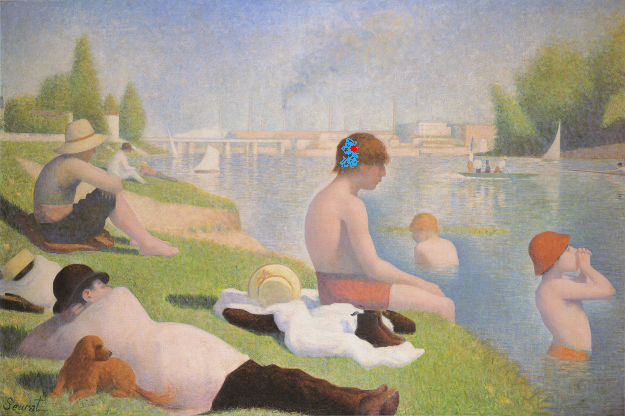
\includegraphics[scale=0.49]{afsnit/vores_implementation/billeder/flood_fill/dot_ff_fixed_10_10}
    \end{center}
    \caption[]{Floodfill-metoden i et billede, med udgangspunkt i en ny
    pixel, hvor der kun sammenlignes med den originale pixel. Den
    tilladte afvigelse er på $(10,10)$.}
    \label{dot_ff_fixed_10_10}
\end{figure}

\begin{figure}[!h]
    \begin{center}
        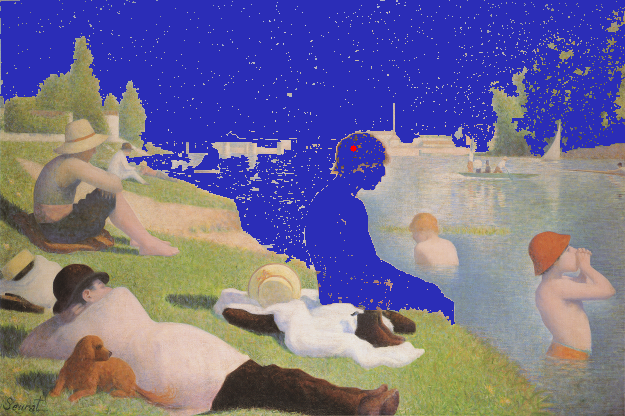
\includegraphics[scale=0.49]{afsnit/vores_implementation/billeder/flood_fill/dot_ff_var_10_10}
    \end{center}
    \caption[]{Floodfill med samme udgangspunkt og afvigelse som i figur
    \ref{dot_ff_fixed_10_10}, men der sammenlignes nu med den nye
    startpixel. Med en større tilladt afvigelse, breder floodfill sig
    meget mere og smelter både himmel, hav og dreng sammen.}
    \label{dot_ff_var_10_10}
\end{figure}

\begin{figure}[!h]
    \begin{center}
        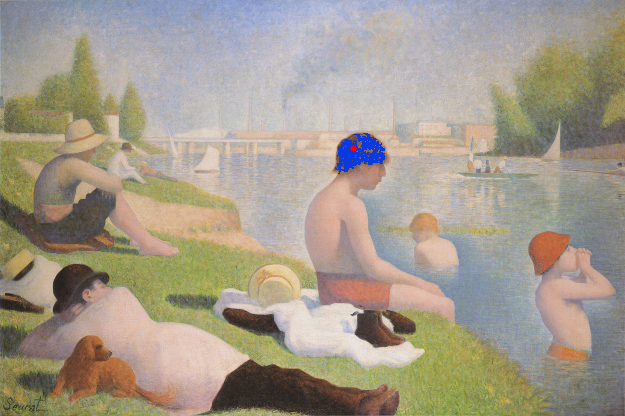
\includegraphics[scale=0.49]{afsnit/vores_implementation/billeder/flood_fill/dot_ff_var_9_9}
    \end{center}
    \caption[]{Floodfill med samme udgangspunkt som i figur
    \ref{dot_ff_fixed_10_10} og \ref{dot_ff_var_10_10}. Her bruges igen
    sammenligning med ny startpixel, men nu med en afvigelse på $9,9$.
    Denne lille ændring er nok til, at vi holder os pænt indenfor den
    region som udgøres af drengens hår.}
    \label{dot_ff_var_9_9}
\end{figure}

\subsubsection{Hvilken metode passer bedst?}
Som nævnt ovenfor, og illustreret i billederne, er der to måder vi kan
bruge floodfill på. Hvis man vælger at regne varianten ud fra den første
startpixel, ses det, at metoden vil indskrænke sig meget og ikke komme
ind i alle hjørner af en region. Til gengæld har denne fremgangsmåde
sværere ved at krydse kanter og på den måde komme ind i en ny region.

Vælger man at ændre varianten efter den nye startpixel, ses det, at man
vil male større regioner. Da denne fremgangsmåde hele tiden tilpasser
varianten, kan man medtage regioner, der langsomt skifter farve. Et godt
eksempel ses i figur \ref{dot_ff_var_10_10}, hvor drengens krop og
bukser bliver set som sammenhængende. Dette er interessant, især med
hensyn til digitale billeder af malerier, da solen eller blitzens
refleksion kan påvirke billedets farver. Af samme grund er den
fremgangsmåde heller ikke særlig følsom over for kanter, hvilket
resulterer i, at man let kommer til at gå ind i andre regioner.

Vi har valgt at benytte os af den sidstnævnte metode, da den efter vores
mening giver det bedste resultat. Vi vurderer, at det er vigtigere at
tage højde for sol og små farveskift end at være sikker på, at vi ikke
går ud over kanterne. Vi vil senere beskrive, hvordan vi på anden vis
sikrer, at vi beholder kanterne.

Som illustreret i billederne skal vi dog stadig tage højde for, hvordan
vi vil sætte tærskelværdierne. Indtil videre bliver de sat efter, hvad
der giver det mest illustrative resultat.

%For at få denne metode til at virke på 25000 billeder, hvor en del af
%billederne ikke har samme farvetone eller er blevet falmet, må der
%for hvert billede udregnes hvad for en varians i farve der skal bruges.

}

% vim: set tw=72 spell spelllang=da:


}

% vim: set tw=72 spell spelllang=da:
